\DocumentMetadata{
	tagging=on,
	pdfstandard = ua-2,
	pdfversion  = 2.0,
	lang        = en-US,
	%testphase   = {math, table, firstaid},
	tagging-setup={
		math/alt/use,
		math/setup=mathml-SE
	}
}

\documentclass[11pt, letterpaper]{article}

% --- Packages for Accessibility and Design ---
\usepackage[T1]{fontenc}
\usepackage[margin=1in]{geometry}
\usepackage[dvipsnames]{xcolor}
\usepackage{graphicx}
\usepackage{tikz}
\usetikzlibrary{arrows.meta, positioning, calc, shapes.geometric}

% --- Color Definitions (Accessible & Professional) ---
\definecolor{MainBlue}{HTML}{003366}
\definecolor{SubBlue}{HTML}{E6F2FF}
\definecolor{DarkGreen}{HTML}{006633}
\definecolor{DarkRed}{HTML}{990000}
\definecolor{LightGreen}{HTML}{E7F4EA}
\definecolor{LightRed}{HTML}{F8E6E6}
\definecolor{AccentGold}{HTML}{B07D00}
\definecolor{NeutralGray}{HTML}{4D4D4D}

\usepackage{tcolorbox}
\tcbuselibrary{breakable, skins}
\usepackage{enumitem}
\usepackage{array}
\usepackage{booktabs}
\usepackage[unicode, colorlinks=true, linkcolor=MainBlue, urlcolor=MainBlue]{hyperref}
\usepackage{bookmark}
\usepackage{amsmath, amssymb}

\graphicspath{{public/}{public/assets/}{public/assets/plots/}}

\hypersetup{
	pdftitle={Accessible Scientific Documents},
	pdfauthor={Author},
	pdfsubject={Example accessible scientific document},
	pdfkeywords={accessibility, tagged PDF, scientific writing, LuaLaTeX}
}

% The current LaTeX lab block-tagging code can report hook-count mismatches
% around breakable tcolorboxes even when the document typesets.
\ExplSyntaxOn
\msg_redirect_name:nnn { tag } { para-hook-count-wrong } { warning }
\ExplSyntaxOff

% --- Helper for Tagged Headings ---
\newcommand{\taggedsection}[1]{\section{\texorpdfstring{\color{MainBlue}#1}{#1}}}
\newcommand{\taggedsubsection}[1]{\subsection{\texorpdfstring{\color{DarkGreen}#1}{#1}}}

% --- Reusable Visual Styles ---
\newtcolorbox{takeawaybox}{
	breakable,
	enhanced,
	colback=SubBlue!45,
	colframe=MainBlue,
	boxrule=0.7pt,
	arc=2pt,
	left=8pt,
	right=8pt,
	top=7pt,
	bottom=7pt
}

\setlist[itemize]{leftmargin=*, topsep=4pt, itemsep=2pt}
\setlist[enumerate]{leftmargin=*, topsep=4pt, itemsep=2pt}

\tikzset{
	process/.style={
		draw=MainBlue,
		fill=SubBlue,
		rounded corners=2pt,
		very thick,
		align=center,
		text width=2.4cm,
		minimum height=1.05cm
	},
	check/.style={
		draw=DarkGreen,
		fill=LightGreen,
		rounded corners=2pt,
		very thick,
		align=center,
		text width=2.3cm,
		minimum height=1.05cm
	},
	warn/.style={
		diamond,
		draw=DarkRed,
		fill=LightRed,
		very thick,
		aspect=2,
		align=center,
		inner sep=1pt,
		text width=2.25cm
	},
	flowarrow/.style={-{Stealth[length=3mm]}, very thick, draw=NeutralGray},
	plotmark/.style={circle, draw=MainBlue, fill=white, very thick, minimum size=4.5pt, inner sep=0pt}
}

% --- Metadata for Title ---
\title{\color{MainBlue}\Huge\bfseries Accessible Scientific Documents\\[0.5cm]
	\large\color{DarkRed} A LuaLaTeX example with tagged structure, math, figures, and references}
\author{Author}
\date{Summer Semester}

% --- Main Document ---
\begin{document}

\maketitle

\tagpdfparaOn

\tableofcontents
\clearpage

\taggedsection{Purpose and Reader Navigation}

This document is a compact starting point for scientific articles, reports, and course notes that should compile to a tagged PDF with LuaLaTeX. It demonstrates structural headings, mathematical notation, tables, vector diagrams, imported raster graphics, cross-references, and a references section.

\begin{takeawaybox}
	An accessible scientific document should expose the same logical organization to assistive technology that sighted readers infer from layout. Use real section commands, captions, labels, alternative text, and meaningful link text rather than relying on visual styling alone.
\end{takeawaybox}

\taggedsubsection{Document Structure}

The section hierarchy is intentionally regular: sections contain subsections, figures have captions, and references are cited in the surrounding prose. For example, Figure~\ref{fig:workflow} gives a high-level authoring workflow, while Table~\ref{tab:checklist} lists checks that are useful before sharing a PDF.

\taggedsubsection{Accessible Scientific Claims}

Scientific writing is easier to navigate when important claims are stated before technical details. A typical result paragraph might read as follows.

\begin{quote}
	The error decreased monotonically for the tested step sizes, and the final residual was below the reporting threshold. The convergence pattern is consistent with the update rule in Equation~\eqref{eq:gradient-update}.
\end{quote}

\taggedsection{Mathematics and Notation}

\taggedsubsection{Displayed Equations}

Use LaTeX math environments rather than raw display delimiters. With the document metadata at the top of this file, the LaTeX tagging layer can attach MathML-oriented alternative representations where supported by the toolchain.

The fundamental theorem of calculus is a simple displayed equation:

\begin{equation}
	\int_a^b f(x)\,dx = F(b)-F(a).
	\label{eq:ftc}
\end{equation}

For a least-squares objective,
\begin{equation}
	J(\theta)=\frac{1}{m}\sum_{i=1}^{m}\left(h_\theta(x_i)-y_i\right)^2,
	\label{eq:objective}
\end{equation}
one common iterative update is
\begin{equation}
	\theta_{k+1}=\theta_k-\alpha\nabla J(\theta_k),
	\label{eq:gradient-update}
\end{equation}
where \(\alpha>0\) is the learning rate.

\taggedsubsection{Lists Near Equations}

When a formula has several symbols, a short list can be clearer than a dense paragraph.

\begin{itemize}
	\item \(m\) is the number of observations.
	\item \(h_\theta(x_i)\) is the model prediction for observation \(i\).
	\item \(y_i\) is the measured response.
	\item \(\nabla J(\theta_k)\) is the gradient evaluated at iteration \(k\).
\end{itemize}

\taggedsection{Tables and Checklists}

\taggedsubsection{A Tagged Table}

\begin{table}[htbp]
	\centering
	\caption{Accessibility checks for a scientific PDF.}
	\label{tab:checklist}
	\tagpdfsetup{table/header-rows={1}}
	\begin{tabular}{>{\raggedright\arraybackslash}p{0.27\linewidth}
			>{\raggedright\arraybackslash}p{0.35\linewidth}
			>{\raggedright\arraybackslash}p{0.25\linewidth}}
		\toprule
		Check & Why it matters & Example in this file \\
		\midrule
		Section hierarchy & Screen readers and PDF outlines use headings for navigation. & Sections and subsections are created with structural commands. \\
		Figure descriptions & Visual information needs a text alternative. & Figures~\ref{fig:workflow}, \ref{fig:descent}, and \ref{fig:tagged-png} include alt text. \\
		Captioned graphics & Captions support citation, review, and cross-reference workflows. & Every figure and table has a caption and label. \\
		Machine-readable math & Mathematical expressions should be exposed beyond visual glyphs. & Equations~\eqref{eq:objective} and \eqref{eq:gradient-update} use equation environments. \\
		References & Citations should be reachable from the prose and listed consistently. & The bibliography cites accessibility and PDF standards \cite{wcag21,pdfua}. \\
		\bottomrule
	\end{tabular}MathML
	\tagpdfsetup{table/header-rows={}}
\end{table}

\taggedsection{Tagged Vector Figures}

\taggedsubsection{Workflow Diagram}

The TikZ picture in Figure~\ref{fig:workflow} uses the `alt' key on the \texttt{tikzpicture} environment. The visual diagram remains available to sighted readers, while the tag structure receives a concise text description of the same content.

\begin{figure}[htbp]
	\centering
	\begin{tikzpicture}[
		alt={Flow diagram showing a four step accessible scientific publishing workflow: draft semantic source, compile with LuaLaTeX tagging, inspect reading order and alternative text, then publish tagged PDF and source files.},
		node distance=1.5cm,
		font=\small
	]
		\node[process] (draft) {\small Draft semantic\\source};
		\node[process, right=of draft] (compile) {\small Compile with\\LuaLaTeX};
		\node[warn, right=of compile] (inspect) {Inspect\\output};
		\node[check, right=of inspect] (publish) {Publish PDF\\and source};

		\draw[flowarrow] (draft) -- node[above, font=\scriptsize] {structure} (compile);
		\draw[flowarrow] (compile) -- node[above, font=\scriptsize] {tags} (inspect);
		\draw[flowarrow] (inspect) -- node[above, font=\scriptsize] {fixes} (publish);

		\draw[flowarrow, bend right=-45] (inspect.south) to node[below, font=\scriptsize] {revise} (draft.south);
	\end{tikzpicture}
	\caption{A workflow for producing an accessible scientific PDF.}
	\label{fig:workflow}
\end{figure}

\taggedsubsection{Plot-Style Figure with Redundant Encoding}

Figure~\ref{fig:descent} uses both color and markers. This avoids encoding essential information by color alone, which is important for readers with color-vision deficiencies and for grayscale printing.

\begin{figure}[htbp]
	\centering
	\begin{tikzpicture}[scale=1.75,
		alt={Contour plot of a bowl-shaped objective function with a marked gradient descent path moving from the upper left toward the minimum near the lower right.}
	]
		\fill[SubBlue!12, rounded corners=4pt] (-3.75,-2.75) rectangle (3.75,2.75);
		\draw[gray!35, rounded corners=4pt] (-3.75,-2.75) rectangle (3.75,2.75);
		\draw[-{Stealth[length=2.5mm]}, thick, draw=NeutralGray] (-3.05,0) -- (3.05,0) node[right, text=NeutralGray] {\(\theta_1\)};
		\draw[-{Stealth[length=2.5mm]}, thick, draw=NeutralGray] (0,-2.0) -- (0,2.15) node[above, text=NeutralGray] {\(\theta_2\)};

		\coordinate (min) at (0.7,-0.4);
		\begin{scope}[rotate around={-18:(min)}]
			\fill[LightGreen!55] (min) ellipse [x radius=0.45cm, y radius=0.27cm];
			\draw[DarkGreen, line width=1.2pt] (min) ellipse [x radius=0.45cm, y radius=0.27cm];
			\draw[AccentGold!85!black, line width=1.1pt] (min) ellipse [x radius=0.95cm, y radius=0.58cm];
			\draw[AccentGold!65!black, thick] (min) ellipse [x radius=1.45cm, y radius=0.9cm];
			\draw[MainBlue!70!black, thick] (min) ellipse [x radius=2.0cm, y radius=1.25cm];
			\draw[MainBlue!45!black, thick] (min) ellipse [x radius=2.6cm, y radius=1.65cm];
		\end{scope}

		\draw[MainBlue, line width=1.35pt, rounded corners=7pt, -{Stealth[length=3mm]}]
			(-2.35,1.55) -- (-1.55,0.95) -- (-0.75,0.42) -- (-0.05,0.02) -- (0.42,-0.22) -- (0.66,-0.35);

		\foreach \point in {
			(-2.35,1.55),
			(-1.55,0.95),
			(-0.75,0.42),
			(-0.05,0.02),
			(0.42,-0.22),
			(0.66,-0.35)
		}{
			\node[plotmark] at \point {};
		}

		\node[font=\scriptsize, text=MainBlue, above left=2pt] at (-2.35,1.55) {start};
		\fill[DarkGreen] (min) circle [radius=2.4pt];
		\node[draw=DarkGreen, fill=white, rounded corners=2pt, inner sep=3pt, font=\scriptsize, text=DarkGreen] (minlabel) at (2.15,-1.35) {minimum};
		\draw[DarkGreen, thick, -{Stealth[length=2mm]}] (minlabel.west) -- (min);
	\end{tikzpicture}
	\caption{A TikZ contour-style diagram with a gradient descent trajectory.}
	\label{fig:descent}
\end{figure}

\taggedsection{Tagged Raster Graphics}

\taggedsubsection{Importing a PNG}

The PNG in Figure~\ref{fig:tagged-png} is imported with \texttt{\textbackslash includegraphics}. The important accessibility detail is the explicit \texttt{alt} option. For complex research figures, keep the caption short and put the full explanation in the surrounding prose or in the alternative text.

\begin{figure}[htbp]
	\centering
	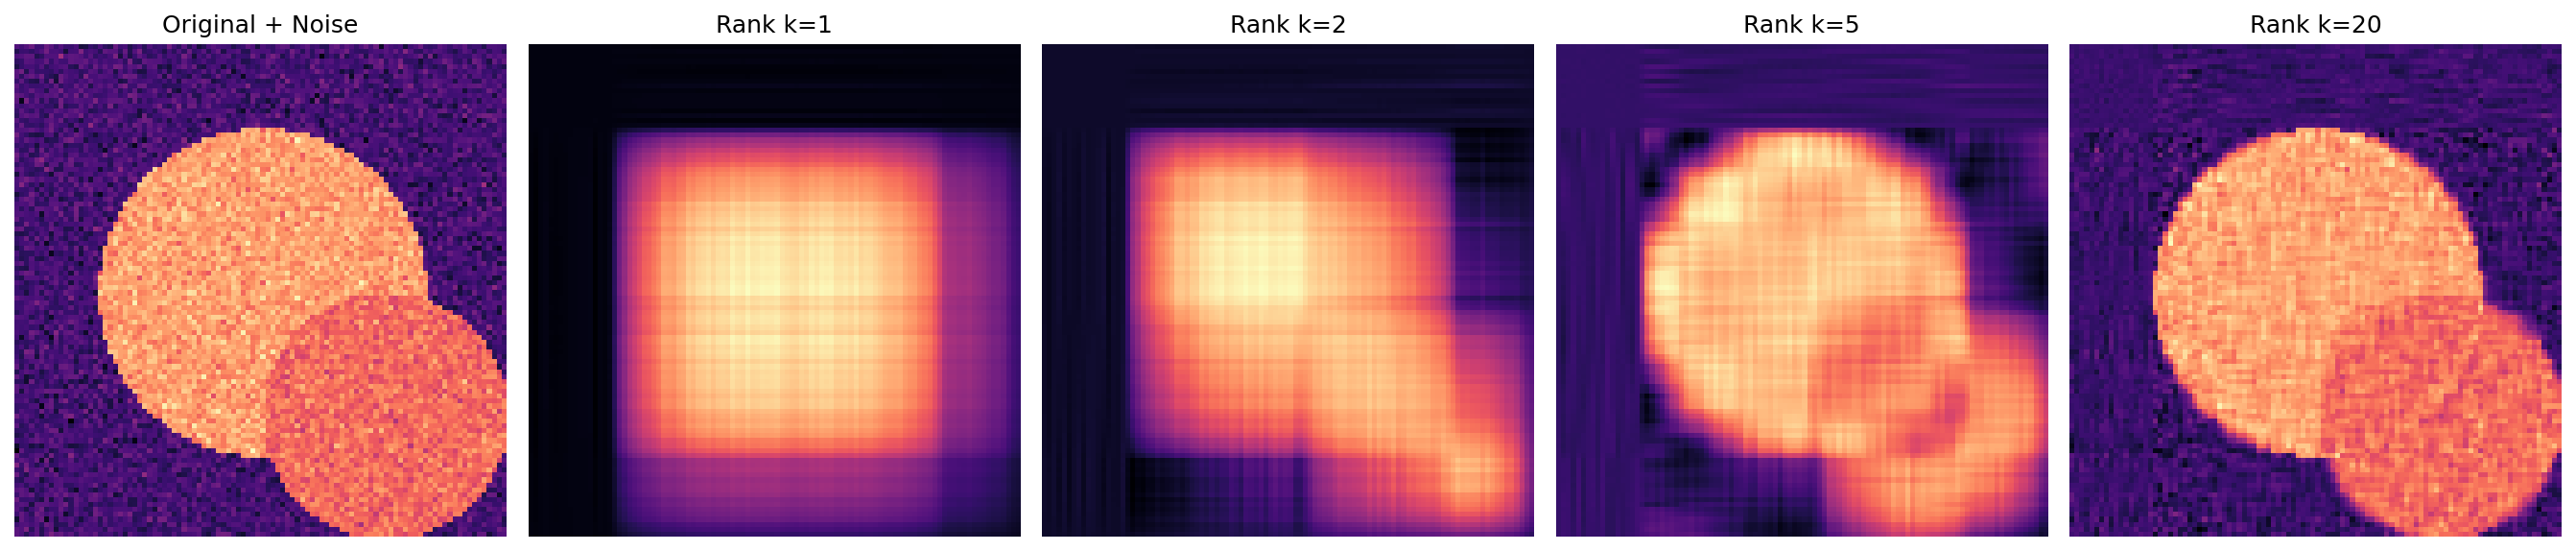
\includegraphics[
		width=\linewidth,
		tag=Figure,
		alt={Wide PNG comparison of low-rank singular value decomposition image reconstructions. The panels progress from coarse reconstructions with few singular values to clearer reconstructions using more singular values.}
	]{assets/svd_compression.png}
	\caption{Imported PNG with explicit alternative text.}
	\label{fig:tagged-png}
\end{figure}

\taggedsubsection{Writing Useful Alternative Text}

Good alternative text should communicate the role of the figure in the argument. It usually does not need to list every visual detail.

\begin{enumerate}
	\item Start with the figure type, such as ``flow diagram,'' ``contour plot,'' or ``SVD reconstruction comparison.''
	\item State the main pattern or conclusion.
	\item Include labels, units, and trends when they are needed to understand the result.
	\item Avoid phrases such as ``image of'' unless the medium is itself relevant.
\end{enumerate}

\taggedsection{Reproducibility Notes}

\taggedsubsection{Source and Output}

For course notes and scientific reports, it is often useful to distribute the tagged PDF together with the source file and any external images. That lets readers audit equations, regenerate figures, and correct accessibility metadata without reverse-engineering the PDF.

\taggedsubsection{Before Sharing}

Before publishing, compile at least twice so the table of contents and cross-references settle. Then inspect the resulting PDF for reading order, document language, title metadata, bookmarks, figure descriptions, and meaningful link text. External validators can help, but they do not replace a manual review of whether the text alternatives are scientifically accurate.

\clearpage

\begin{thebibliography}{9}

\bibitem{wcag21}
World Wide Web Consortium.
\newblock \emph{Web Content Accessibility Guidelines (WCAG) 2.1}.
\newblock W3C Recommendation, 2018.

\bibitem{pdfua}
International Organization for Standardization.
\newblock \emph{ISO 14289-2:2024, Document management applications -- Electronic document file format enhancement for accessibility -- Part 2: Use of ISO 32000-2 (PDF/UA-2)}.
\newblock ISO, 2024.

\bibitem{latexcompanion}
Frank Mittelbach, Michel Goossens, Johannes Braams, David Carlisle, and Chris Rowley.
\newblock \emph{The LaTeX Companion}.
\newblock Addison-Wesley, second edition, 2004.

\end{thebibliography}

\end{document}
